%%%%%%%%%%%%%%%%%%%%%%%%%%%%%%%%%%%%%%%%%
% Journal Article
% LaTeX Template
% Version 2.0 (February 7, 2023)
%
% This template originates from:
% https://www.LaTeXTemplates.com
%
% Author:
% Vel (vel@latextemplates.com)
%
% License:
% CC BY-NC-SA 4.0 (https://creativecommons.org/licenses/by-nc-sa/4.0/)
%
% NOTE: The bibliography needs to be compiled using the biber engine.
%
%%%%%%%%%%%%%%%%%%%%%%%%%%%%%%%%%%%%%%%%%

%----------------------------------------------------------------------------------------
%	PACKAGES AND OTHER DOCUMENT CONFIGURATIONS
%----------------------------------------------------------------------------------------

\documentclass[
	letterpaper, % Paper size, use either a4paper or letterpaper
	10pt, % Default font size, can also use 11pt or 12pt, although this is not recommended
	unnumberedsections, % Comment to enable section numbering
	twoside, % Two side traditional mode where headers and footers change between odd and even pages, comment this option to make them fixed
]{LTJournalArticle}

\addbibresource{bibliography.bib} % BibLaTeX bibliography file

\runninghead{CVE-2017-0144 EternalBlue} % A shortened article title to appear in the running head, leave this command empty for no running head

\footertext{\textit{Report1 } (MICS CYBER 204, Summer-2024)} % Text to appear in the footer, leave this command empty for no footer text

\setcounter{page}{1} % The page number of the first page, set this to a higher number if the article is to be part of an issue or larger work

%----------------------------------------------------------------------------------------
%	TITLE SECTION
%----------------------------------------------------------------------------------------

\usepackage[title,toc,titletoc]{appendix}
\usepackage{titlesec}
\usepackage{lscape}

\title{EternalBlue CVE-2017-0144 \\ MICS-204 Report 1, Summer 2024} % Article title, use manual lines breaks (\\) to beautify the layout

% Authors are listed in a comma-separated list with superscript numbers indicating affiliations
% \thanks{} is used for any text that should be placed in a footnote on the first page, such as the corresponding author's email, journal acceptance dates, a copyright/license notice, keywords, etc
\author{
	Karl-Johan Westhoff \\
	email \href{mailto:kjwesthoff@berkeley.edu}{kjwesthoff@berkeley.edu}
}

% Affiliations are output in the \date{} command
\date{UC Berkleley School of Information \\
MICS Course 204 Summer 2024
}

% % Full-width abstract
% \renewcommand{\maketitlehookd}{%
% 	\begin{abstract}
% 		\noindent Lorem ipsum dolor sit amet,rta porttitor.
% 	\end{abstract}
% }

%----------------------------------------------------------------------------------------

\begin{document}

\maketitle % Output the title section

%----------------------------------------------------------------------------------------
%	ARTICLE CONTENTS
%----------------------------------------------------------------------------------------

\section{Introduction}
EternalBlue \cite[CVE-2017-0144]{CVE-2017-0144} vulnerability has all the traits of a superstar hack, it was probably discovered and developed into a tool by NSA, found and leaked by hackers and quickly thereafter used in some of the worst and most destructive malware attacks the world has seen. \\
\newline
EternalBlue first appeared in a leak\cite{Rapid7-on-S0hadow-Broker-Leak} from a hacker group named "The Shadow Brokers"\cite{shadowBrokers-wiki} (TSB) who published a bunch of zero day exploits they claimed to have stolen from the NSA's "Equation Group \footnote{Nickname for NSA’s Tailored Access division (TAO). Darknet Diaries \cite{Darknet-Diaries-ep53} has an excellent episode on the shadowBrokers leak}"\cite{kaspersky-eq-group} (None of this has been confirmed). \\
\newline
EternalBlue enables the attacker to launch a shell on the target with windows system privileges. \\
\newline
As the vulnerability is in the Microsoft Server Message Block (SMB) protocol, which enables file shares across different users, locations and networks (When you share a folder or access a networks drive, SMB is used) it is not contained by network architecture such as subnets but s able to roam free based on how SMB is managed typically on a corporate network. EternalBlue, giving an attacker a system shell \footnote{The DoublePulsar tool, also leaked in the shadowBrokers release is a part of EternalBlue and runs 'exec' in 'kernel mode' on the target}, in combination with credentials stealing malware e.g Mimikatz, gives the possibility for some highly potent malware to be crafted, which indeed happened (WannaCry, NotPetya etc.). This leaves EternalBlue as the most expensive software vulnerability - yet. 



\section{Exploits} 

The vulnerability was investigated from by Zian et.al. in \cite{Zian}. Furthermore "zerosum0x0" did a presentation on how EternalBlue works at DefCon26 \cite{zerosum0x0-defcon26} and in \cite{h3xduck} "h3xduck" did a walkthough (All of which i found useful) \\


EternalBlue is a consequence of three features/bugs in version 1 of the SMB protocol (SMBv1) \cite{Koczwara-medium} : 

\begin{enumerate}
	\item{ \textbf{Buffer Overflow} caused by a typecasting error when casting requests from different Windows filesystems}
	\item{ \textbf{Unchecked packages} when sending secondary messages memory is allocated based on sender (attacker) controlled offset allowing allocation of memory}
	\item{ \textbf{"Heap Spraying"} is possible: Data can be written to specific places in memory allowing for code to be inserted and executed}
\end{enumerate}


SMB runs on TCP port 445, i.e. the  exploit works on a port that needs to be open on the firewall (if you want windows file shares to work).
When sending files over the network the SMB protocol uses transactions, where information such as packet size, purpose (the protocol has "special features" such as directory searching etc.) and a list of "File Extended Attributes" (FEAlist) is exchanged in a handshake (SMB Primary Request/Interim Response in Figure \ref{fig:SMB-transaction}). 
\newline{}
SMB allows for transferring large files where the transaction is split up requiring secondary packets to be send (SMB Transaction Sec. Request 1-N in Figure \ref{fig:SMB-transaction}). Large file transfers make it easier to hide suspicious packets.  
\newline
The FEAlist and secondary packets are important for the exploit.


\begin{figure} % Single column figure
	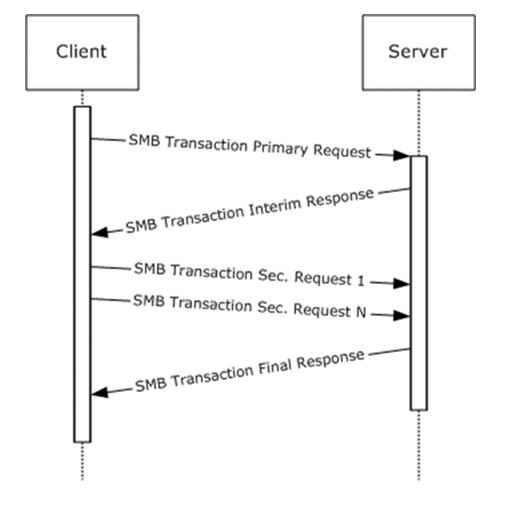
\includegraphics[width=\linewidth]{SMB-transaction.png}
	\caption{Request response, SMB protocol. Source: windows learning }
	\label{fig:SMB-transaction}
\end{figure}

\subsection{How it Works}

\subsubsection{Buffer Overflow}
The FEAlist is a list of key/value properties which are sent with the transactions. 

\begin{itemize}
	\item The client calculates the size of the FEAlist part of the transaction and sends it to the server with the transaction.  
	\item The server allocates space in memory for the FEAlist, using pointer offsets based on the size of the list (it does not keep a 'list' variable)
	\item The size of the list is provided by the client, and checked by the server and re-calculated if the size dos not match. However, 
	\begin{itemize}
		\item There are multiple versions of the FEAlist format depending on the filesystem used (OS/2 vs NT). And there is a bug in the conversion of FEAlist file size between OS/2 and NT (bug in a function called "SrvOs2FeaListSizeToNt" in srv.sys \cite{h3xduck}) where only half the memory is allocated when sending a OS/2 formatted FEAlist - a 16 byte 'int' is cast to a 8 byte 'short' resulting in a buffer overflow see Ghidra analysis of code from \cite{h3xduck} in Appendix Figure \ref{fig:Ghidra_srv.sys}. 
	\end{itemize}
\end{itemize}


\subsubsection{Secondary Transactions, Heap Grooming}
When the transaction size is large, SMB splits it into subsequent transactions, see Figure \ref{fig:SMB-transaction}. The client provides the packet size, which is used as offset for memory allocation i.e. the client (attacker) decides where data is stored in memory. The packets of data are kept as "non-paged" by srv.sys on the heap until all the secondary packets have arrived, this is indicated with a flag in the last packet (again the attacker controls that). 

In Figure \ref{fig:SMB-transaction} 'Transaction Sec.' requests can be submitted until the 'N'th' packet containing the end flag. The system does not check the format of the packets, there are 2 different kinds: 'COM' and 'NT' each with their own secondary packets, the protocol assumes the packet format to be that of the final packet send, therefore it is possible to mix the OS and NT packets. And send the first packet as 'NT' with the incorrect FEAList size followed by a subsequent 'OS' type packets. This allows for sending secondary OS packages with the FEAList buffer overflow 'feature' (if we were sending OS only, the double 16bit FEAList would not be allowed)
\newline
In appendix a Wireshark dump recorded during exploit is shown. The transaction starts with NT \footnote{"NT Trans Request"} and subsequent transactions are of OS type \footnote{"Trans2 Secondary Request"}.      

\subsubsection{Placement of code - From Remote}
The last thing needed is to place a payload where functions are executed on the stack. Windows has the "Windows Hardware Abstraction Layer (HAL)" which runs in kernel mode and has a static address \cite{h3xduck} which can be exploited to execute code.  
\newline  
In between Sec. Request 1-N in Figure \ref{fig:SMB-transaction} a new handshake for a new transaction can be 'weaved in' \footnote{"Session Setup AndX"} while keeping the stream of secondary packets flowing (See \nameref{Appendix} Figure \ref{fig:wiresharkDump} Wireshark dump packet No.135 Session "Setup and X process" started before the first transaction FID0X0000 is finished in No.168).     

The second transaction is placed in the spots freed, this can be manipulated using the buffer overflows to happen at the address of HAL - now the attackers code runs...         

\section{Remediation} 

\subsection{Fix the buffer overflow}
Patching this was super simple (change the 8bit short to a 16bit int in the "SrvOs2FeaListSizeToNt" in srv.sys, see Appendix Figure \ref{fig:Ghidra_srv.sys}) - the problem is as always to get the patch rolled out.
The patch MS2017-010 was issued March 14, 2017 \cite{MS2017-010} before EternalBlue was published April 14, 2017 \cite{enwiki:1219364760} by shadowBrokers (speculation is that NSA nudged Microsoft after being aware that the leak was imminent, they had kept it secret for a long time before that, and the vulnerability showed up before)

\subsection{Randomize HAL's location}
Newer version of Windows uses Address Space Layout Randomization (ASLR) for the HAL process, which makes it impossible to predict and control where packages land in memory based on the offsets. 

\subsection{Sandbox processes on the OS}
Maybe these application layer interactions with the network should be sandboxed out of the heap so there is no memory cross talk possible. 


\section{Conclusion}
In hindsight it is obvious to target the SMB protocol as a backdoor. The protocol works close to the operating system (memory is allocated directly on the heap with system privileges), the protocol is designed to be lightweight in terms of package checks and balances (the memory is allocated based on sender specified offsets) Presumably all of this is done to make the transfer of files feel as close to a local operation as possible. Later versions ( > 1) of SMB had removed the 'extra' messages used by EternalBlue and were not affected, but at the time systems kept the earlier SMB versions in the stack for backwards compatibility, in fact a recommendation against EternalBlue is to disable version 1 of SMB.       



%----------------------------------------------------------------------------------------
%	 REFERENCES
%----------------------------------------------------------------------------------------

\printbibliography % Output the bibliography

%----------------------------------------------------------------------------------------



%----------------------------------------------------------------------------------------
%	 Appendices
%----------------------------------------------------------------------------------------


\clearpage
\begin{appendices}
\onecolumn
\appendix
\section{Appendix} \label{Appendix}

\subsection{Buffer Overflow Bug in srv.sys}
A figure from \cite{h3xduck} with code deconstructed from a vulnerable windows srv.sys is shown in Figure \ref{fig:Ghidra_srv.sys}
\newline
Note line 27 the variable “param1” is being casted from an integer (dword) pointer to a short (word). Then in that word the subtraction of itself with another variable piVar1 is stored. Thus we are essentially casting into a short the result of the subtraction of two integers \cite{h3xduck}.



\begin{figure}[ht] % Single column figure
	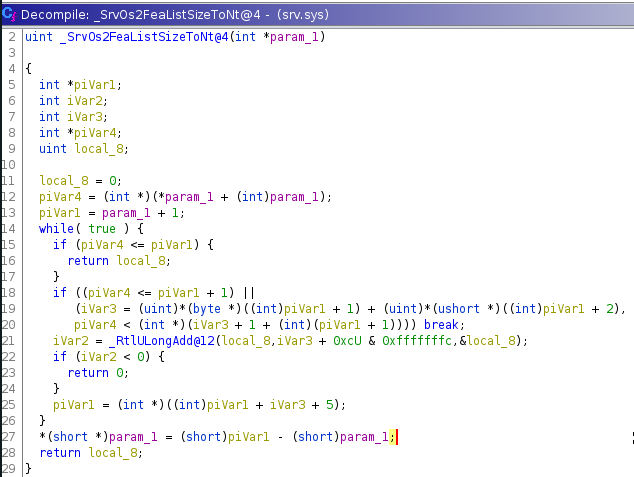
\includegraphics[width=\linewidth]{GhidraOfSrv.png}
	\caption{The buffer overflow in Srv!SrvOs2FeaToNt, deconstructed using Ghidra, figure from \cite{h3xduck}}
	\label{fig:Ghidra_srv.sys}
\end{figure}



\subsection{Demo using Metasploit}
As a demonstration of how easily the EternalBlue vulnerability can be deployed to get a system shell using Metasploit, I ran the exploit on virtual machines locally on my computer:
\subsubsection[short]{Attacer machine} Kali linux running Metasploit (see Figure \ref{fig:metasploit-pawned}).



\subsubsection[short]{Target machine}
Early Windows 7 machine (2009) see Figure \ref{fig:ExploitableWin7}, the exploit is proven to work up to 2017 where a patch was introduced (MS17-010).
Only modification is that a folder was shared on the desktop with 'user' permissions (this opens the necessary outbound rules on the firewall)

\begin{figure}[ht] % Single column figure
	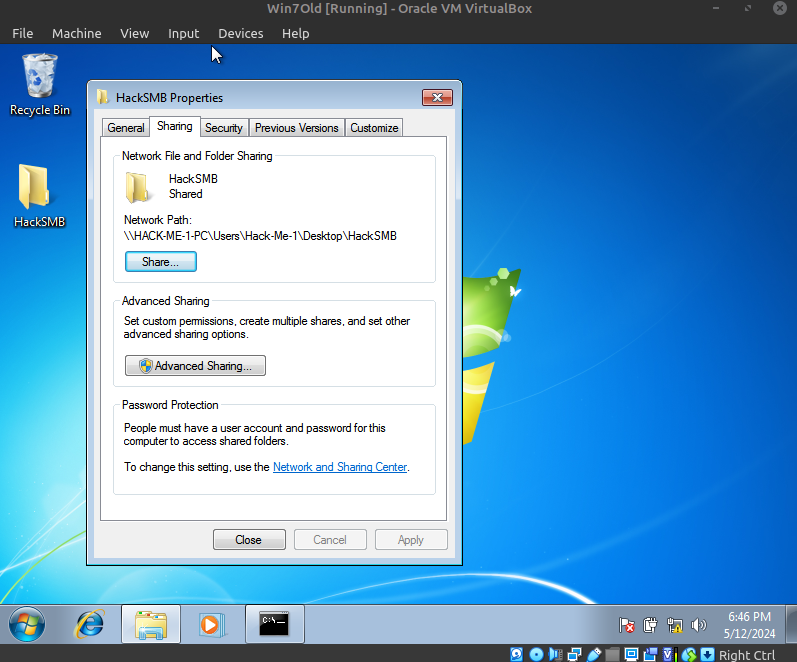
\includegraphics[width=\linewidth]{ExploitableWin7.png}
	\caption{Exploited windows 7 2009 service pack 1}
	\label{fig:ExploitableWin7}
\end{figure}

\begin{figure}[ht] % Single column figure
	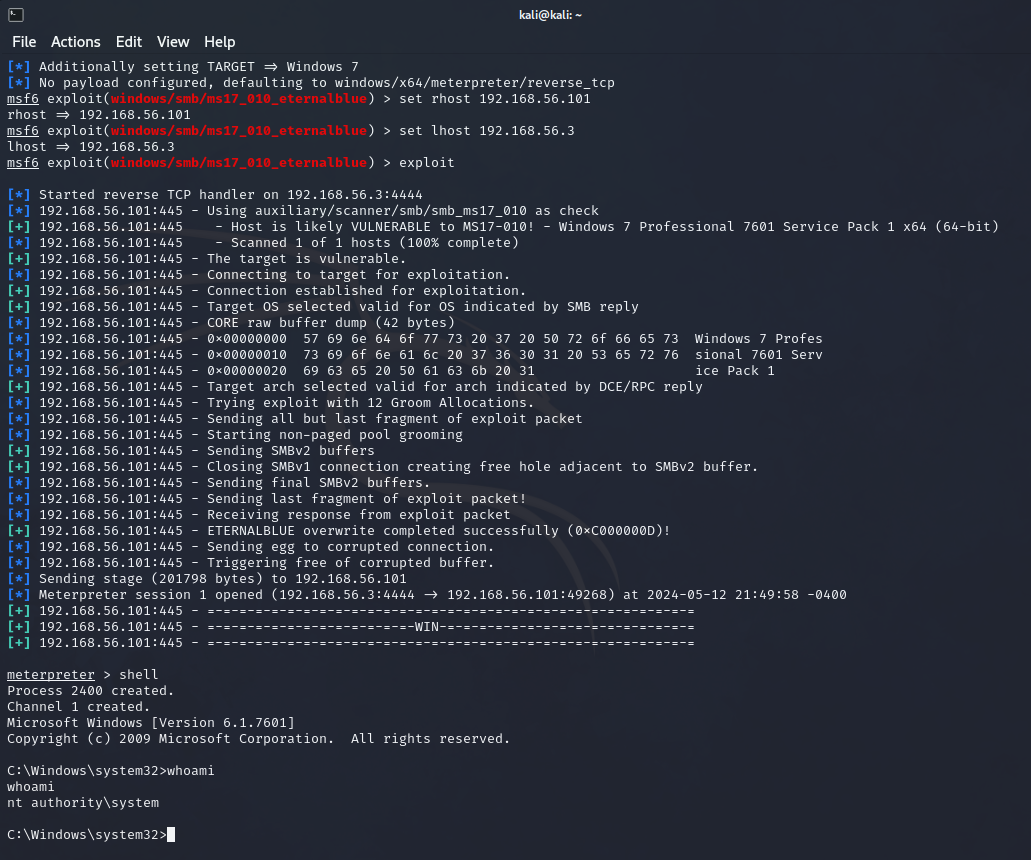
\includegraphics[width=\linewidth]{metasploit-pawned.png}
	\caption{Very easy with Metasploit}
	\label{fig:metasploit-pawned}
\end{figure}


\subsubsection{Wireshark dump}
Wireshark dump recorded during exploit is shown in Figure \ref{fig:wiresharkDump}, where the transaction starts with NT "NT Trans Request" No.44 and subsequent Transactions are of OS type "Trans2 Secondary Request" No.47-64. In between a new session is started "Session Setup AndX" No.135 and finally the first transaction is terminated in No.168 	     


\begin{landscape}
\begin{figure}[ht] % Single column figure
	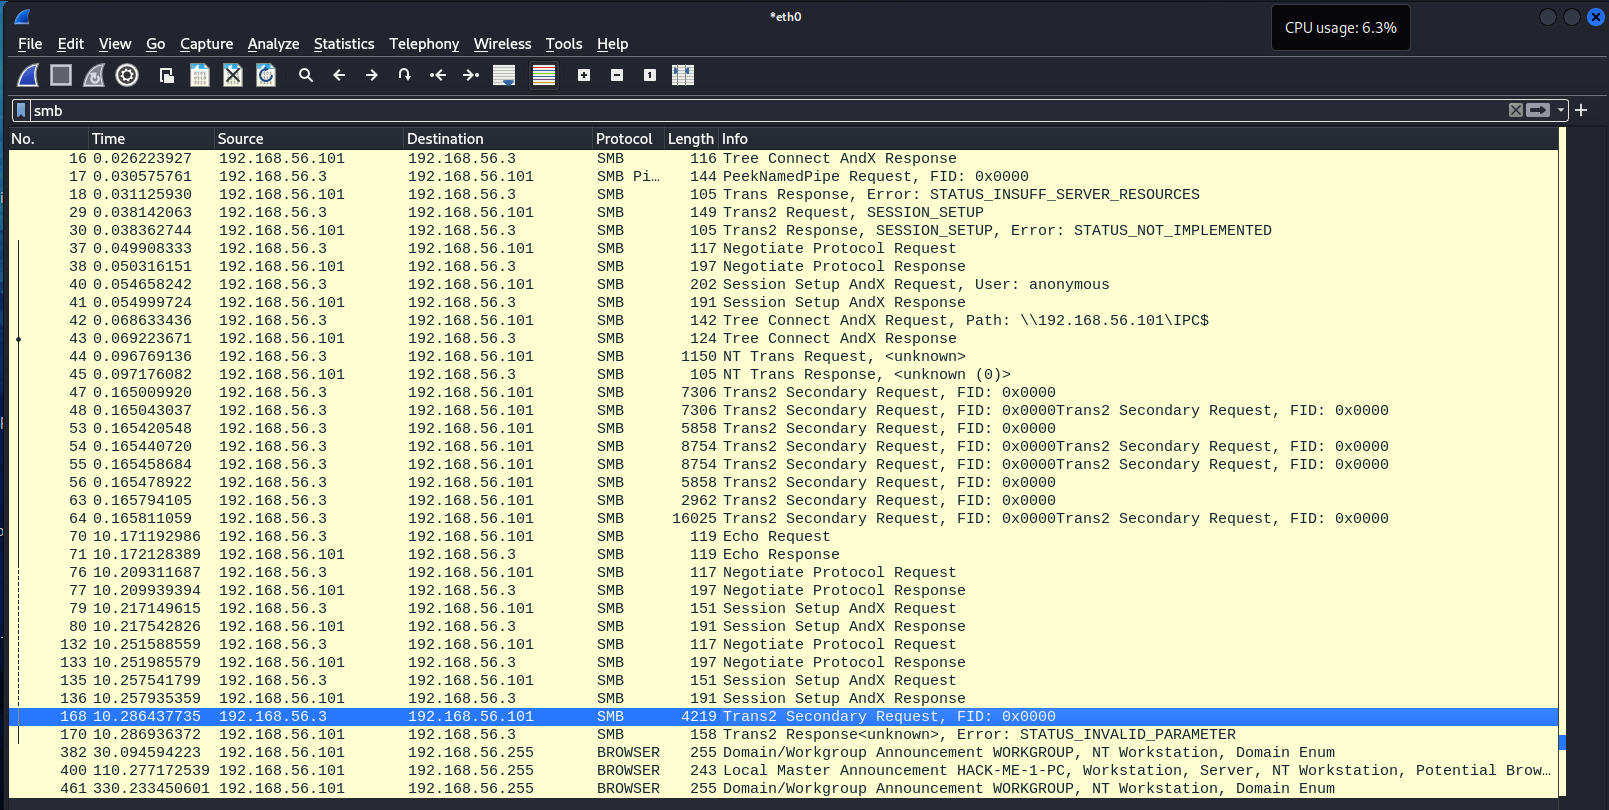
\includegraphics[width=\linewidth]{WiresharkEternalBlue.png}
	\caption{SMB Traffic during exploit}
	\label{fig:wiresharkDump}
\end{figure}
\end{landscape}

\end{appendices}



% sudo nmap -sV 10.10.10.40  

% sudo nmap --script smb-os-discovery -p445 10.10.10.40

% sudo nmap --script smb-enum-shares -p445 10.10.10.40 


% msfconsole

% use windows/smb/ms17_010_eternalblue
% set RSHOST and LHOST

% poke around using meterpreter



% Section 5 (Optional): Appendix – include the exploit code here if you’d like to. Do NOT include the full exploit source code in Section 2


% \begin{equation}
% 	\cos^3 \theta =\frac{1}{4}\cos\theta+\frac{3}{4}\cos 3\theta
% 	\label{eq:example}
% \end{equation}

% Automatically referencing an equation number using its label: Equation \ref{eq:example}.


%------------------------------------------------








% \section{Methodologies}

% \subsection{Sample Sites \& Processing}

% This line shows how to use a footnote to further explain or cite text\footnote{Example footnote text.}.

% This is a bullet point list:

% \begin{itemize}
% 	\item Arcu eros accumsan lorem, at posuere mi diam sit amet tortor
% 	\item Fusce fermentum, mi sit amet euismod rutrum
% 	\item Sem lorem molestie diam, iaculis aliquet sapien tortor non nisi
% 	\item Pellentesque bibendum pretium aliquet
% \end{itemize}

% Mauris interdum porttitor fringilla. Proin tincidunt sodales leo at ornare. Donec tempus magna non mauris gravida luctus. Cras vitae arcu vitae mauris eleifend scelerisque. Nam sem sapien, vulputate nec felis eu, blandit convallis risus. Pellentesque sollicitudin venenatis tincidunt. In et ipsum libero. Nullam tempor ligula a massa convallis pellentesque.

% This is a numbered list:

% \begin{enumerate}
% 	\item Donec dolor arcu, rutrum id molestie in, viverra sed diam
% 	\item Curabitur feugiat
% 	\item Turpis sed auctor facilisis
% \end{enumerate}

% \subsection{Species Identification}


%------------------------------------------------

% \section{Results}

% \begin{table} % Single column table
% 	\caption{Example single column table.}
% 	\centering
% 	\begin{tabular}{l l r}
% 		\toprule
% 		\multicolumn{2}{c}{Location} \\
% 		\cmidrule(r){1-2}
% 		East Distance & West Distance & Count \\
% 		\midrule
% 		100km & 200km & 422 \\
% 		350km & 1000km & 1833 \\
% 		600km & 1200km & 890 \\
% 		\bottomrule
% 	\end{tabular}
% 	\label{tab:distcounts}
% \end{table}

% Referencing a table using its label: Table \ref{tab:distcounts}.

% \begin{table*} % Full width table (notice the starred environment)
% 	\caption{Example two column table with fixed-width columns.}
% 	\centering % Horizontally center the table
% 	\begin{tabular}{L{0.2\linewidth} L{0.2\linewidth} R{0.15\linewidth}} % Manually specify column alignments with L{}, R{} or C{} and widths as a fixed amount, usually as a proportion of \linewidth
% 		\toprule
% 		\multicolumn{2}{c}{Location} \\
% 		\cmidrule(r){1-2}
% 		East Distance & West Distance & Count \\
% 		\midrule
% 		100km & 200km & 422 \\
% 		350km & 1000km & 1833 \\
% 		600km & 1200km & 890 \\
% 		\bottomrule
% 	\end{tabular}
% \end{table*}

% \begin{figure} % Single column figure
% 	\includegraphics[width=\linewidth]{Tolmukapea.jpg}
% 	\caption{Anther of thale cress (Arabidopsis thaliana), fluorescence micrograph. Source: Heiti Paves, \href{https://commons.wikimedia.org/wiki/File:Tolmukapea.jpg}{https://commons.wiki-\\media.org/wiki/File:Tolmukapea.jpg}.}
% 	\label{fig:tcanther}
% \end{figure}

% Referencing a figure using its label: Figure \ref{fig:tcanther}.


% \begin{figure*} % Two column figure (notice the starred environment)
% 	\includegraphics[width=\linewidth]{Fibroblastid.jpg}
	% \caption{Bovine pulmonary artery endothelial cells in culture. Blue: nuclei; red: mitochondria; green: microfilaments. Computer generated image from a 3D model based on a confocal laser scanning microscopy using fluorescent marker dyes. Source: Heiti Paves, \href{https://commons.wikimedia.org/wiki/File:Fibroblastid.jpg}{https://commons.wikimedia.org/wiki/File:Fibroblastid.jpg}.}
% 	\label{fig:bpartery}
% \end{figure*}


% \subsection{Links}

% This is a clickable URL link: \href{https://www.latextemplates.com}{LaTeX Templates}. This is a clickable email link: \href{mailto:vel@latextemplates.com}{vel@latextemplates.com}. This is a clickable monospaced URL link: \url{https://www.LaTeXTemplates.com}.

%------------------------------------------------

% \section{Discussion}

% This statement requires citation \autocite{Smith:2023qr}. This statement requires multiple citations \autocite{Smith:2023qr, Smith:2024jd}. This statement contains an in-text citation, for directly referring to a citation like so: \textcite{Smith:2024jd}.

% \subsection{Subsection One}

% Suspendisse potenti. Vivamus suscipit dapibus metus. Proin auctor iaculis ex, id fermentum lectus dapibus tristique. Nullam maximus eros eget leo pretium dapibus. Nunc in auctor erat, id interdum risus. Suspendisse aliquet vehicula accumsan. In vestibulum efficitur dictum. Sed ultrices, libero nec fringilla feugiat, elit massa auctor ligula, vehicula tempor ligula felis in lectus. Suspendisse sem dui, pharetra ut sodales eu, suscipit sit amet felis. Donec pretium viverra ante, ac pulvinar eros. Suspendisse gravida consectetur urna. Pellentesque vitae leo porta, imperdiet eros eget, posuere sem. Praesent eget leo efficitur odio bibendum condimentum sit amet vel ex. Nunc maximus quam orci, quis pulvinar nibh eleifend ac. Quisque consequat lacus magna, eu posuere tellus iaculis ac. Sed vitae tortor tincidunt ante sagittis iaculis.

% \subsection{Subsection Two}

% Nullam mollis tellus lorem, sed congue ipsum euismod a. Donec pulvinar neque sed ligula ornare sodales. Nulla sagittis vel lectus nec laoreet. Nulla volutpat malesuada turpis at ultricies. Ut luctus velit odio, sagittis volutpat erat aliquet vel. Donec ac neque eget neque volutpat mollis. Vestibulum viverra ligula et sapien bibendum, vel vulputate ex euismod. Curabitur nec velit velit. Aliquam vulputate lorem elit, id tempus nisl finibus sit amet. Curabitur ex turpis, consequat at lectus id, imperdiet molestie augue. Curabitur eu eros molestie purus commodo hendrerit. Quisque auctor ipsum nec mauris malesuada, non fringilla nibh viverra. Quisque gravida, metus quis semper pulvinar, dolor nisl suscipit leo, vestibulum volutpat ante justo ultrices diam. Sed id facilisis turpis, et aliquet eros.

% \subsubsection{Subsubsection Example}

% Duis venenatis eget lectus a aliquet. Integer vulputate ante suscipit felis feugiat rutrum. Aliquam eget dolor eu augue elementum ornare. Nulla fringilla interdum volutpat. Sed tincidunt, neque quis imperdiet hendrerit, turpis sapien ornare justo, ac blandit felis sem quis diam. Proin luctus urna sit amet felis tincidunt, sed congue nunc pellentesque. Ut faucibus a magna faucibus finibus. Etiam id mi euismod, auctor nisi eget, pretium metus. Proin tincidunt interdum mi non interdum. Donec semper luctus dolor at elementum. Aenean eu congue tortor, sed hendrerit magna. Quisque a dolor ante. Mauris semper id urna id gravida. Vestibulum mi tortor, finibus eu felis in, vehicula aliquam mi.

% Aliquam arcu turpis, ultrices sed luctus ac, vehicula id metus. Morbi eu feugiat velit, et tempus augue. Proin ac mattis tortor. Donec tincidunt, ante rhoncus luctus semper, arcu lorem lobortis justo, nec convallis ante quam quis lectus. Aenean tincidunt sodales massa, et hendrerit tellus mattis ac. Sed non pretium nibh. 

% Donec cursus maximus luctus. Vivamus lobortis eros et massa porta porttitor. Nam vitae suscipit mi. Pellentesque ex tellus, iaculis vel libero at, cursus pretium sapien. Curabitur accumsan velit sit amet nulla lobortis, ut pretium ex aliquam. Proin eget volutpat orci. Morbi eu aliquet turpis. Vivamus molestie urna quis tempor tristique. Proin hendrerit sem nec tempor sollicitudin.


\end{document}
